\begin{figure}[tbp]
\centering
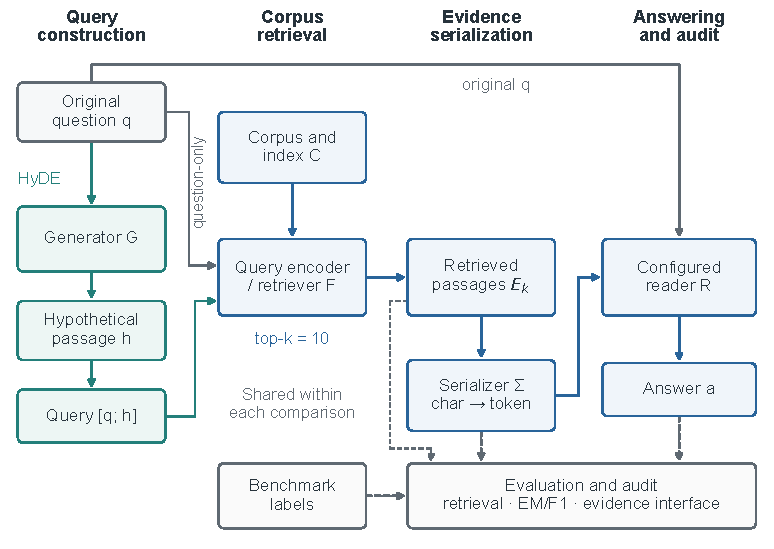
\includegraphics[width=\textwidth]{Fig1_Workflow.pdf}
\caption{System workflow and evidence boundary. Question-only and HyDE are separate conditions sharing the corpus, index, retrieval configuration and top-$k=10$ within each comparison. HyDE forms $[q;h]$ from the question $q$ and hypothetical passage $h$. The reader receives the original question and serialized corpus evidence under condition-specific character and token budgets. Solid arrows show inference; dashed arrows show evaluation and audit. Benchmark labels enter evaluation only. Optional answer postprocessing is omitted.}
\label{fig:method_pipeline}
\end{figure}
